%-------------------------------------------------------
\section{Distributing Intelligence}
%-------------------------------------------------------

Given the current interpretation and use of the AA and DT abstractions in the literature, it is apparent that both AAs and DTs can be used to encapsulate some form of intelligence. 
%(the former have been conceived to do this), and both have been used to model and engineer IoT systems and applications (the latter in particular).
Thus, an open engineering question involving both research communities is: \textbf{are AAs and DTs different ways to achieve essentially the same thing? 
Are they (possibly partially) overlapping? 
Or are they complementary?} 

In this section, we argue for the latter. 
We object that existing approaches often blur the boundaries between the responsibilities of AAs and DTs creating confusion by trying to fit everything within the same abstraction (be it an AA, a DT, or any other unprincipled \emph{ad-hoc} combination of the two abstractions). 
%
The direct cause for this is that the AA and DT abstractions are not associated with clear roles within the architecture of an IoT system, hence they do not help produce \emph{modular} and \emph{reusable} designs that can then be implemented across application domains. 
%
This generates several competing architectural models all trying to address similar problems and thus overlapping with existing solutions, leading to fragmentation and confusion for researchers and practitioners seeking the ``best'' design for their specific problem at hand. 

In an attempt to remedy this, 
we first identify a set of principles to assist system designers in the analysis of the functional requirements of their intelligent IoT system at hand (Subsection~\ref{ssec:principles}), 
then frame AAs and DTs as the two abstractions perfectly adhering to such principles, complementarily (Subsection~\ref{ssec:abs-def}). 
Finally, we propose AAs and DTs as the basic building blocks that designers can use and compose to create their application-specific software architectures (Subsection~\ref{ssec:multi-layer}).


%======================================================
\subsection{Design Principles}
\label{ssec:principles}
%======================================================

%Recent literature tried to shed light on the distinguishing traits of the two abstractions/paradigms of AAs and DTs, to motivate their synergistic exploitation in dealing with the engineering of IoT systems and applications.
%
We take our move from the quite abstract software engineering criterion of \emph{separation of concerns}given in~\cite{DBLP:conf/atal/MarianiPR22}, expanding and refining it along three dimensions to make it more practically useful: \emph{specificity}, \emph{scope}, and \emph{time}. 
%
These are meant to be used to analyse the requirements posed by the intelligent functionalities summarised in Subsection~\ref{ssec:functions}. 
%
%Subsection~\ref{ssec:abs-def} discusses how they define a spectrum of design choices leaning towards a DT, an AA, or some integration of both.
We anticipate that it is likely that neither of these dimensions \emph{alone} is sufficient to determine \emph{univocally} which abstraction is best suited for a given functionality. 
Instead, we argue that they all need to be taken into consideration together when approaching the design of an intelligent IoT system.
%
%Even though we are now going to present them separately, it is important to keep in mind that they are %not meant to be a strict set of rules to be followed blindly, but 
%a set of principles that can guide designers in the analysis of a DI system when used together.


The reason to ground our principles in a \emph{software engineering} standpoint, 
that is, from the perspective of the software designer of an IoT system or application, 
is that IoT systems are increasingly no longer ``mostly hardware'' ones, with interconnected devices that simply exchange data. 
Instead, they are increasingly becoming complex cyberphysical systems
where software plays a prominent role, 
especially regarding endowing intelligence into devices (hence into the system).
There, thus, proper engineering of the software layer of the overall IoT deployment 
is crucial to guarantee both functional and non-functional properties. 
Not by chance, the publications discussed in Section~\ref{sec:back} deal mostly with \emph{software} engineering, architectures, and design. 


%--------------------------------------
\subsubsection{Specificity} 
%--------------------------------------

The first principle we propose is what we call \emph{specificity}, whose spectrum is depicted in Figure~\ref{fig:specificity}, and is defined informally as 
\begin{quote}
    ``how much a given (intelligent) functionality is \emph{specifically} serving a given application goal (at one end of a spectrum), rather than being \emph{generally} exploitable by multiple goals and potentially across application scenarios (at the other end)''.
\end{quote}
%
With this, we want to help IoT systems and application designers to distinguish between 
\emph{(i)} those features that are strictly tied to the achievement of a specific \emph{application goal}, and 
\emph{(ii)} those that may instead be \emph{generically} useful to pursue multiple goals and build other intelligent functionalities and/or applications on top. 
%
This is especially important for designing highly modular systems. 
%
%Separating these functionalities effectively is crucial to identify components that can more easily evolve over time and at the same time can support the evolution of the whole system allowing new functionalities to be added on top.

\begin{figure}[!b]
    \centering
    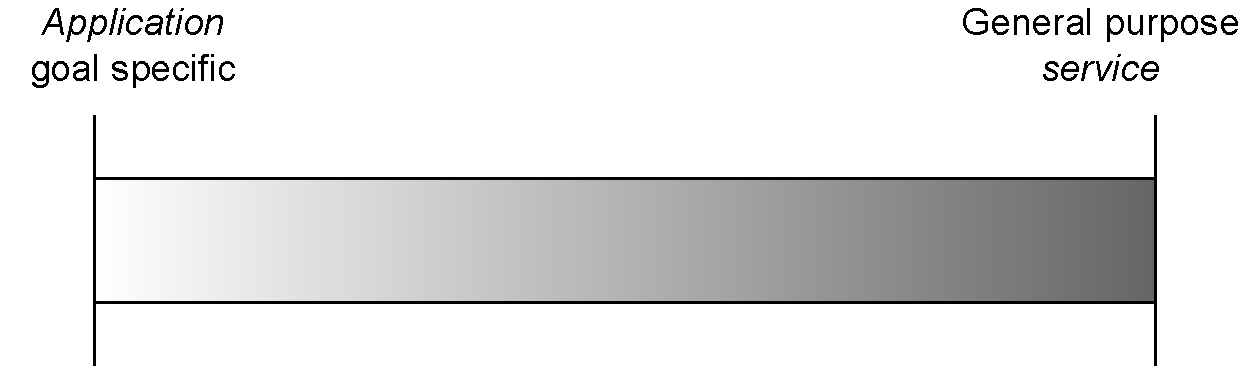
\includegraphics[width=.6\columnwidth]{figures/dt-mas/specificity-spectrum.pdf}
    \caption{The spectrum of \emph{specificity}: from intelligent functionalities specific to an application goal to general-purpose services.}
    \label{fig:specificity}
    %\Description{the spectrum of specificity principle, with a gradient from specific to general}
\end{figure}

In IoT systems, for instance, a widespread general-purpose functionality concerns the digitalization of Physical Assets (PAs) to enable intelligent functionalities such as prediction of that assets' future states, and simulation of alternate states. 
%
%This is an essential step as it allows the collection of data from the devices and the exposure of the operations that can be invoked by other components. 
%
Functionalities like these can be considered to be not tied to the application goals, but to the general services offered by the IoT platform, in an open systems, ``as-a-service'' perspective~\cite{10.1145/3507909}. 
%
In contrast, functionalities such as fault diagnosis or inference of specific information may be relevant only in the context of the application domain or goal. 
Another example would be the implementation of adaptive control policies and decision-making strategies: these are likely to be specialised for the system at hand, as they encode the requirements and goals set by stakeholders. 

However, each specific instance of these categories of intelligent functionalities devised out in Subsection~\ref{ssec:functions} must be carefully examined by the system designer in light of this (and the other) principle(s), as there can be no ``rule of thumb'' generally applicable to every application domain and goal. 
%
%For instance, in a smart building, there could be several policies introduced to optimize comfort or energy consumption. Those policies will be part of the system due to a specific requirement coming from the stakeholders which means that even if they are reusable across different buildings they have been designed. 
%
%However, we want to stress that deciding whether these functionalities can be considered potentially general, instead, as they can output results that can be used by different components in the system, is up to the system designer. 
%He/she must keep our proposed guiding principle in mind, match it against the functionality to be realised (and its requirements), and then find the appropriate answer to the question of specificity. 
%
%Also, keep in mind that taking a single principle in isolation is unlikely to completely determine a design choice in complex IoT systems and applications. 
%That's why we provide more, complementary principles. 
%
Also, generally speaking, there may be edge cases that may feel ``in violation'' of our proposed principles but are actually not.  
For instance, it may be the case that an application goal coincides with the digitalisation of an asset for prediction purposes. 

This case should not be interpreted as ``wrong'' because it defines a prediction function as application-specific. 
On the contrary, the specificity principle, in this specific case, cannot guide designers' choice \emph{alone}. 
This is one reason to propose more, complementary principles, that better capture the different nuances of complex systems and applications---not by chance the edge case described is quite simple. 

%-----------------------------------------
\subsubsection{Scoping} % Locality, Scoping, Coupling 
%-----------------------------------------

%\ste{Tutti}{Abbiamo convenuto che il nocciolo del principio sta nel capire da dove/cosa viene l'input alla funzione: se locale a una entità di interesse o se globale da più entità opportunamente aggregate}

%\ste{Tutti}{ruolo centrale della modellazione: il DT modella una realtà di interesse (PA) ben specifica e concettualmente delimitata, mentre l'agente modella obiettivi applicativi e criteri decisionali che possono avere legame mutevole con la realtà modellata utile allo scopo. I secondi sfruttano i primi come servizio, per non costringere l'agente a modellare la realtà (meglio dirlo in sez. 4.2 forse). Questo abilita il riuso: il DT può essere usato in più applicazioni se offre servizi generici, l'agente può lavorare su più domini grazie a DT che astraggono (anche questo meglio dirlo in sez. 4.2 forse).}

The second principle we propose, we call \emph{scoping}, is defined as follows:
\begin{quote}
    ``to what extent a given (intelligent) functionality requires data from the whole system (at one end of a spectrum) or a single individual entity of interest (at the other end) to deliver its results''
\end{quote}
With this, we want to help IoT systems and applications designers distinguish between \emph{(i)} the features that require data, inputs, and interactions with multiple entities of interest in the system at hand (up to \emph{global} information, synthesised at the system level), and \emph{(ii)} the features that instead require only considering a single asset (the extreme case of \emph{local} information). 
Figure~\ref{fig:scope} depicts this spectrum. 

\begin{figure}[!b]
    \centering
    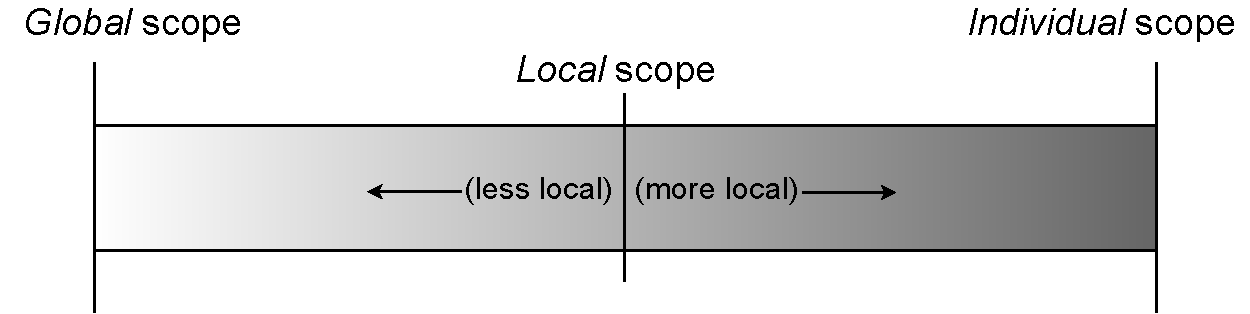
\includegraphics[width=.6\columnwidth]{figures/dt-mas/scope-spectrum.pdf}
    \caption{The spectrum of \emph{scoping}: from intelligent functionalities requiring knowledge of the whole system, to those confined to individual assets.}
    \label{fig:scope}
   
\end{figure}

In any IoT system, due to its inherent connection with the physical world, there are software components whose main function 
is coupled with PAs, which set boundaries to the \emph{scope} within which intelligent functionalities operate. 
For example, by collecting local information only (e.g.\ prediction of the future states of specific machinery, not others). 
%
Conversely, many other functionalities may require a broader scope that goes well beyond such local boundaries. 
%
If we take as an example the domain of a smart home, we can have 
software components that mirror, and grant access to, the individual devices (e.g.\ for remote monitoring and control), 
but also adaptive control routines spanning multiple devices or even multiple rooms to orchestrate a coordinated action (e.g.\ preparing for the comeback of an inhabitant by activating the A/C, unlocking the doors, raising the curtains, etc.). 
%
Accordingly, with the scoping principle, we suggest that system designers consider where the knowledge and data required to accomplish the intelligent function come from, as well as which entities will be subject to its effects. 
%


It should be noted that the \emph{individual} and \emph{global} scopes are the two extremes of the spectrum depicted in Figure~\ref{fig:scope}. 
Functionalities may require data from multiple entities, but such entities may be confined in a limited space, for instance geographically, or network-wise. 
Or, it could be the case that data is required from different and distant entities that are anyway somehow easy to access together---think of overlay networks. 
%
In this case, the proposed principle is still useful to guide design choices, as it forces designers to clarify and sort out why and how they deem the scope to be worth defining global or local (or even individual). 


%--------------------------------------
\subsubsection{Timing} 
%--------------------------------------

The third (and last, for the time being) principle we propose is what we call \emph{timing}, which we define informally as 
\begin{quote}
    ``how much a given functionality relies on any one notion of \emph{time} (e.g.\ physical or logical) to be either explicitly (i.e.\ \emph{time-aware}) or implicitly (i.e.\ \emph{time-situated}) available''% or, not at all
\end{quote}
%
By ``time-aware'', we mean that the functionality requires access to time-related information, either to make it directly observable to consumers of such functionality or to work properly. 
For instance, time series forecasting (a form of prediction) needs an explicit representation of time to be available, hence it is time-aware. 
By ``time-situated'', instead, we mean that the functionality has some dependency on any one notion of time, but such dependency need not be explicitly captured and managed. 
For instance, real-time monitoring and control of an asset surely depend on time, but such a dependency need not be modelled to deliver the functionality. 
Simply, its existence suffices for the functionality to work properly.
There are also some other cases where time does not matter from the designer's standpoint, as time is not an issue when implementing the functionality---e.g., sending commands to an actuator device. 
This whole spectrum is depicted in Figure~\ref{fig:timing}. 

\begin{figure}[!t]
    \centering
    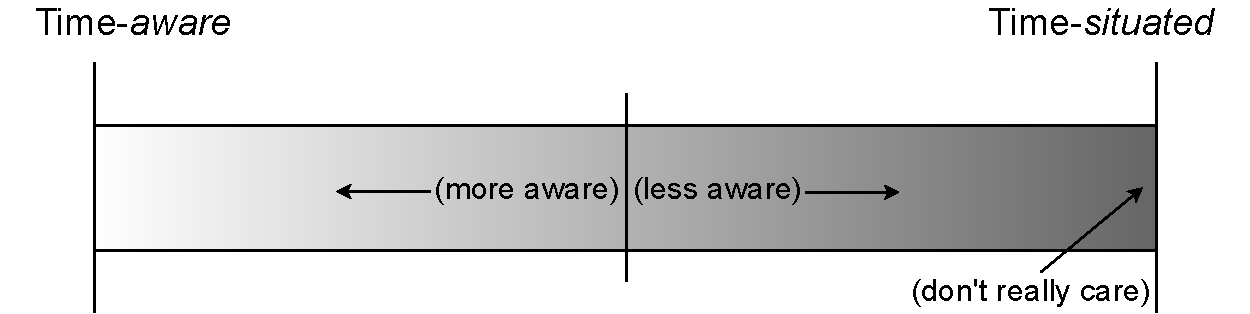
\includegraphics[width=.6\columnwidth]{figures/dt-mas/timing-spectrum.pdf}
    \caption{The spectrum of \emph{timing}: from intelligent functionalities requiring explicit modelling of physical or logical time, to those that don't care.}
    \label{fig:timing}
\end{figure}

Of course, placing intelligent functionalities within this spectrum cannot be a precise operation, as with the other principles. 
But some general considerations about the categories of intelligent functionalities devised in Section~\ref{ssec:functions} can and should be made to aid system designers. 
%
For example, prediction, simulation, and diagnosis are likely to require time awareness. 
How far into the future should an event or state of interest be predicted? 
How long into the future should a simulation extend? 
Conversely, when did a chain of faults lead to the present faulty situation? 
%
Other functionalities, such as inference, learning, and adaptation, may be less demanding and simply be time-situated. 
Of course adaptation actions are based on some events that happened, or on some predicted future state, and need to be carried out in the future, but possibly they do not require an explicit representation of time to work properly as simply their sequential ordering is sufficient to eventually react accordingly. 

%======================================================
\subsection{AAs and DTs as first-class abstractions}
\label{ssec:abs-def}
%======================================================

%\ste{Tutti}{da un lato ci sono le funzionalità, dall'altro le due astrazioni, i nostri princpipi dovrebbero stare in mezzo e tracciare il percorso dalla funzionalità all'astrazione (come quei giochini della sala giochi dove metti le monete in 1 foro in alto e quelle si incanalano in tanti fori in basso, ma rovesciata---le funzionalità sono più fori, le astrazioni meno)}

In the previous subsection, we propose our design principles guided by the intelligent functionalities that are described in the related literature discussed in Section~\ref{sec:back}. 
Now we match such principles against AAs and DTs, to conceptually assess which abstraction is best suited for which end of the spectrum described above for a given principle. 
Figure~\ref{fig:principles} shows the exemplary functionalities and how they are better encapsulated by AAs or DTs according to our principles. 

\begin{figure}[!t]
    \centering
    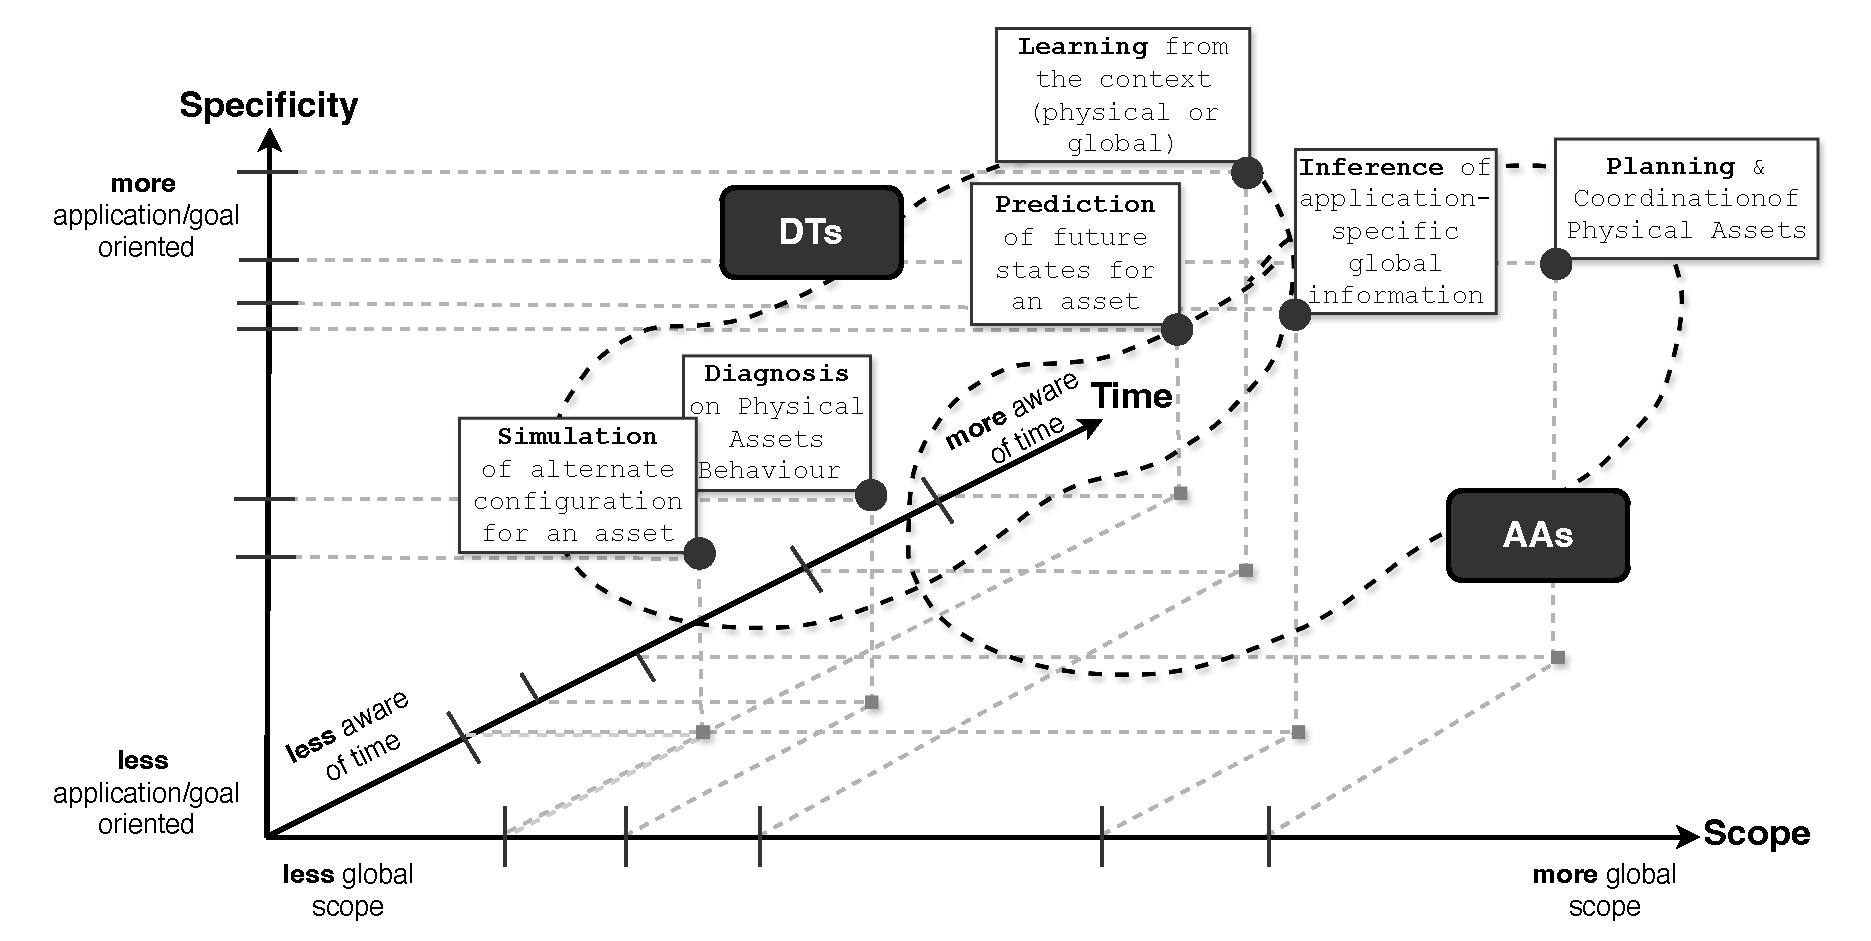
\includegraphics[width=\columnwidth]{figures/dt-mas/principles-aa-dt.pdf}
    \caption{Exemplary intelligent functionalities placed within the spectrum of our design principles. AAs and DTs are clustering those functionalities that they better match with, according to such principles.}
    \label{fig:principles}
    %\Description{A graph with three corresponding to the principles and the main categories of functionalities placed within it, two dotted lines represent an area for which DTs or AAs are more suitable}
\end{figure}

Let us start by considering how AAs and DTs have been used in the \emph{specificity} design principle. 
%\begin{itemize}
%\item 
AAs, being by definition \emph{goal-driven} entities, are usually exploited to encapsulate intelligent functionalities that are strictly related to the problem to solve, hence to the domain and objectives of the application~\cite{DBLP:books/daglib/0077762}. 
%\item 
DTs, instead, are usually exploited with the scope of digitalising assets to provide data-oriented services to consumer applications, \emph{servitisation} being one of their core characteristics~\cite{the-digita-twin-Crespi-2023}. 
%\end{itemize}
The principle of specificity, thus, would encourage designers to encapsulate intelligent functionalities closely matching application goals in AAs, and, complementarily, to model general-purpose services as DTs instead. 

Consider now the \emph{scoping} design principle. 
%\begin{itemize}
%\item 
AAs are not tied to any particular source of information in achieving their goals. 
Although part of the definition of AA includes a relationship with the notion of an environment in which AAs are \emph{situated}~\cite{DBLP:journals/ker/WooldridgeJ95}, AAs are not limited in any particular way to any given ``object'' in such an environment. 
In other words, the application environment (physical or digital) in its entirety is a source of information that AAs can perceive and (possibly) affect---their \emph{global} scope. 
%
%\item 
DTs, instead, are specifically defined as being \emph{coupled} with the individual asset in the physical world that they are digitally representing (their physical twin). 
It is thus natural to give DTs a \emph{local} scope, limited to the information available from this physical asset. 
%\end{itemize}
Note that we deliberately choose the term ``scoping'' instead of, for instance, ``locality'', to avoid the misunderstanding that such design principle is inherently tied with some notion of space, such as in a geographical sense or limited by a physical size boundary under which something can be considered local or not.
%
%We simply mean that there should be a clear boundary in terms of how many physical assets are involved with the intelligent functionality that designers are considering. 
%If an individual asset is the source of information for that functionality, it could be suited to be encapsulated by a DT. 
%Otherwise, if the information needed belongs to multiple sources, an AA might be more conceptually aligned.
%%
%However, the boundary of an individual asset can extend to be a rather large entity.
%%
%In a smart home, for instance, we can envision an asset to be an individual device, a room, or the whole house even. 
%Also, nothing prevents an asset from being a composition of multiple others that have a smaller local boundary. 

Finally, let us position AAs and DTs with respect to the \emph{timing} design principle. 
%\begin{itemize}
%\item 
AAs do not include any explicit notion of time in their definition. 
The situatedness feature already mentioned includes the temporal dimension but does not prescribe agents to capture and model time-related aspects. 
Hence AAs are \emph{time-situated} entities, naturally. 
%\item 
DTs, complementarily, are specifically requested to keep in synch %(shadow)
their related PA to provide an updated digital representation in a timely manner. 
This implies explicitly capturing the time at which events in the PA happened, and modelling the temporal evolution of the PAs. %---such as in threading. 
DTs are thus naturally \emph{time-aware}. 
%\end{itemize}

Summarising the above considerations, AAs and DTs can be described as playing the following roles in the design of distributed intelligent functionalities in IoT systems and applications:
\begin{itemize}
    \item \textbf{AAs} are the components of the IoT system that encapsulate the system/application \textbf{goals}, hence are aware of such specific goals and strive to achieve them by autonomously deciding \textbf{whose other entity} to interact in the whole application domain. 
    AAs are also not particularly tied to any specific notion of time. 
    \item \textbf{DTs}, instead, model and encapsulate properties, behaviours, and functions of specific portions of the IoT system or application domain, therefore are \textbf{inherently bound to specific assets}, to provide \textbf{general-purpose services} to other components or directly to the application. 
    Due to such modelling, DTs must at least account for the specific \textbf{notion of time} relevant to the modelled asset. 
\end{itemize}
%We devise these definitions by observing what are the features that are closer to how Digital Twins and agents have been used about the principles that we identified before and when both have been used for a given dimension we decided to distinguish them to make them complementary rather than keeping them overlapped.
%
We emphasise that these definitions are not meant to set crisp boundaries amongst AAs and DTs in any possible use case and scenario. 
%
Consequently, there is a degree of flexibility in how these definitions can be interpreted to distribute responsibilities across different components.
%
However, having well-defined criteria that dictate how to exploit AAs and DTs as complementary abstractions helps to identify responsibilities in the design of an IoT system willing to fully leverage distributed intelligence.
%
%Furthermore, complementarity is key to leveraging the defining features of each component for the definition of complex behaviour.

To better illustrate this flexibility, the next subsection describes some architectural solutions that can arise from these design principles to deliver different intelligent functionalities in the IoT. 
Furthermore, Section~\ref{sec:case-study} discusses a practical case study, applying the principles to analyse the system requirements.


%======================================================
\subsection{From ``macro'' to ``micro'' architectures}
\label{ssec:multi-layer}
%======================================================

%\ste{Ste}{Besides, what is the architecture of AA? In my view, the architecture of AA is the so-called FCBPSS architecture of a system, see the literature \cite{DBLP:journals/eis/WangWDFKIZ16,DBLP:journals/eis/ZhangW16}. These literatures take a system perspective to a broad manufacturing system, at enterprise level, shopfloor level, etc.
%The authors may want to discuss the modeling of AA with FCBPSS in the future work.}

% \ste{Ste}{1. ora dai principi deriviamo possibili architetture a seconda delle funzionalità attese; 
    % 2. prima 1:1 poi contemplando MAS e multi-DT; 
    % 3. poi chiariamo che ogni ``blocco'' architetturale (lettera) può essere composto a piacere; 
    % 4. da qualche parte ci posizioniamo rispetto a lavori EMAS e WoDT (loro guardano al sistema top-down, noi bottom-up)}

The proposed design principles and their match against AAs and DTs help decide whether an AA or a DT is best suited for a given intelligent functionality. 
However, they tell little about how to combine AAs and DTs \emph{synergistically} when intelligent functionality requires it. 
For instance, because it is positioned within the spectrum of each principle in a way that does not perfectly match all the features of either an AA or a DT, but some of both. 
Accordingly, this section discusses the several ``micro-architectures'' for AAs and DTs integration that may arise during the application of our principles---while the next section provides a practical example for a selection of them. 
We use the term \emph{micro-architecture} ($\mu$-arch, for short) to emphasise an important distinction our architectural perspective has concerning the related literature, discussed below.

The goal of clarifying integration architectures is also witnessed in recent literature, although from different perspectives.
% 
Reference~\cite{DBLP:conf/atal/MarianiPR22} enumerates different alternative architectures to integrate AAs and DTs, depending on the goal of the integration itself. 
%
In~\cite{DBLP:conf/emas/MarianiPR23} the goal is to achieve a technical integration between specific technologies to increase the level of abstraction toward the set of concepts most familiar to the developers of AA. 
%
Another effort, the \emph{Web of Digital Twins} (WoDT) vision~\cite{10.1145/3507909}, 
sees DTs as entities interlinked in a \emph{web of semantic, dynamic relationships}, 
working as the digital substrate that enables structuring a dynamic application domain.
%
According to the WoDT vision, 
a layer of networked DTs works as the interface between applications
(either agent-oriented or not)
and the physical environment they must cope with, 
thus decoupling the two layers and possibly providing augmented and cross-domain functionalities.

Common to these and other architectural proposals in the literature~\cite{iiot_dt_architectural_aspects,guinard2010resource,laghari-2016,Guth2016,Cavalcante2015} is the \emph{top-down}, ``macro-architecture'' perspective adopted: what is proposed is a reference architecture for a whole system, a blueprint to adopt in any given IoT scenario (and beyond).
%
For instance, in the field of enterprise systems architecture, the rise of IoT and the relevance of CPSs in general as the ``backbone'' of many intelligent functionalities within the company (that require asset monitoring and control first and foremost), nurtured research in new designs and methodologies supporting IoT-related goals. 
There, the general trend is to adopt a \emph{System of Systems} (SoS) perspective over the whole enterprise, decomposing the requirements along the same application-agnostic dimensions. 
The FCBPSS architecture is an example \cite{DBLP:journals/eis/WangWDFKIZ16}, where the many systems supporting operations of an enterprise are seen in terms of Functions, Context, Behaviour, Principles (guiding the design), Structure (components realising the function and their relations), and State. 
These very same concepts are applied recursively for the whole enterprise integration system---indeed, a SoS.
%
In contrast, here we propose a bottom-up approach, where the architecture of the overall system is the result of the composition of multiple $\mu$-arch, depicted in Figure~\ref{fig:architecture} by making use of the following components: 
%
%\begin{itemize}
%\item 
Physical Assets (``PA'' squares), which represent the entities in the real world (e.g. devices, objects, people, processes, organisations) that the IoT system needs to model; 
%\item 
DTs (``DT'' circles); 
%\item 
AAs (``A'' circles); 
%\item 
and the intelligent functionalities (the 3D boxes), which may be entire applications or simply one of the many functions needed for the application at hand. 
%\end{itemize}
\begin{figure}[!t]
    \centering
    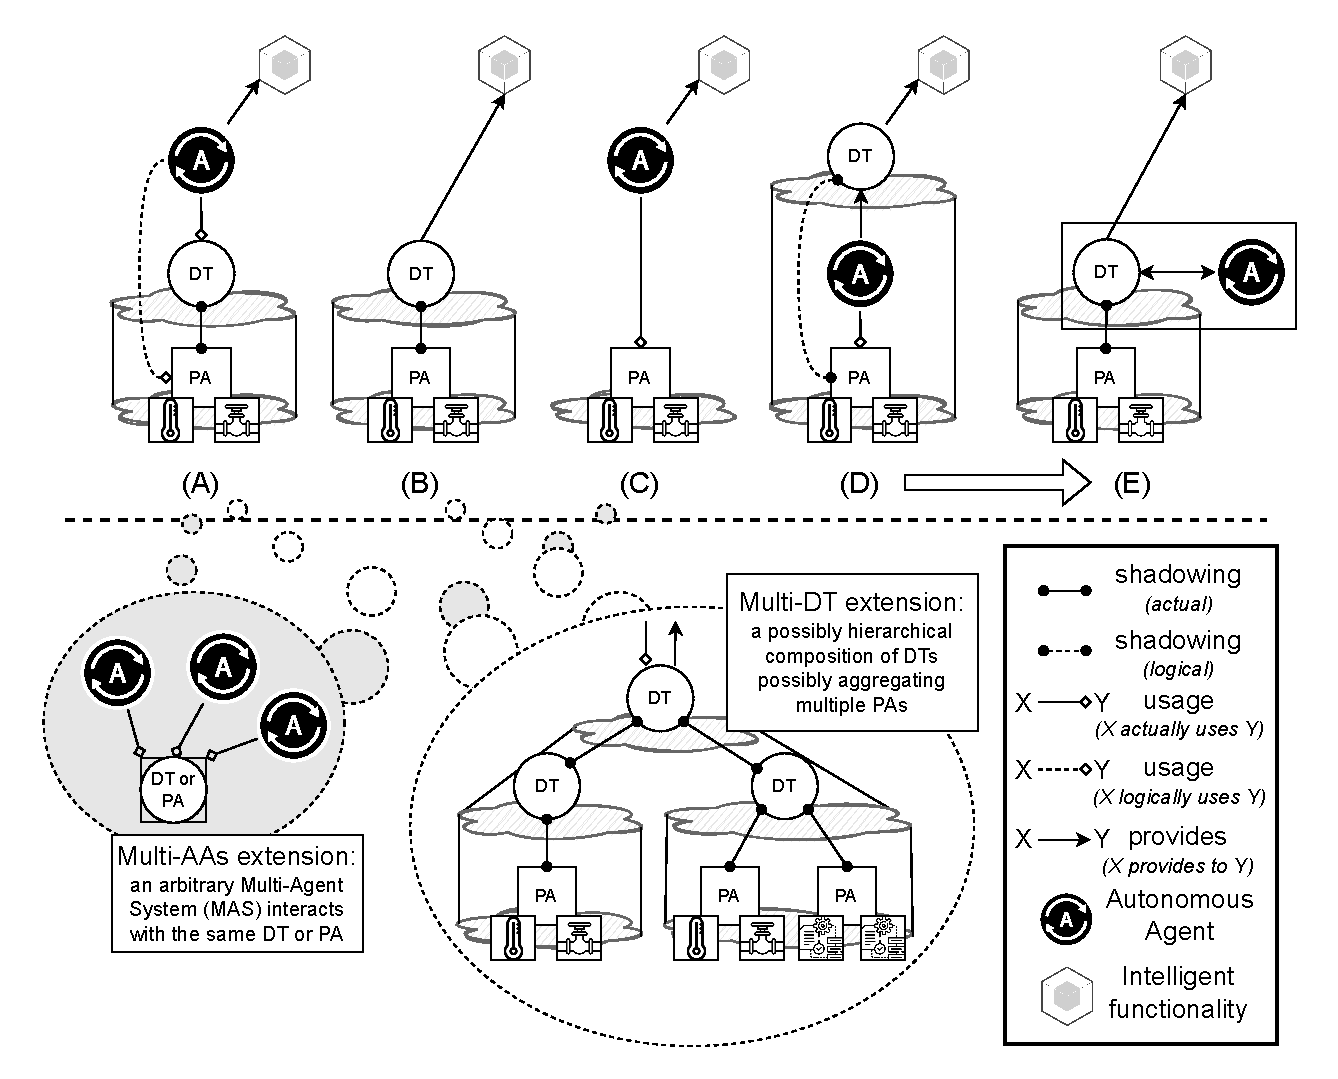
\includegraphics[width=\columnwidth]{figures/dt-mas/2024-toit-si-architecture-aa-dt.pdf}
    \caption{Architectural perspective for the synergistic combination of AAs and DTs in distributing intelligence in IoT systems. Each letter denotes a specific \emph{micro-architecture} that may arise from the application of our principles. Such architectures can be combined to give shape to the overall system architecture, in a bottom-up way.}
    \label{fig:architecture}
\end{figure}
%
The possible $\mu$-archs are: 
%
\begin{itemize}
    \item $\mu$-arch \textbf{(A)} is the most common in the related literature already mentioned~\cite{DBLP:conf/atal/MarianiPR22,DBLP:conf/emas/MarianiPR23,10.1145/3507909}, and it is widely used as a reference architecture for the integration of AAs and DTs~\cite{DBLP:conf/atal/MarianiPR22}. 
    There, the intelligent functionality to realise neither perfectly matches an AA nor a DT. 
    For instance, it could have high specificity, require time-awareness, and a scope locally extended to a set of related PAs. 
    Hence, PAs are digitalised by DTs, that offer services to AAs encapsulating the intelligent functionalities directly serving the applications' goals. 
    %
    This is the typical $\mu$-arch that arises when a given intelligent functionality can be decomposed into an application-specific part and a PA-specific part~\cite{DBLP:conf/atal/MarianiPR22}. 
    The former can request to complement the PA-related information with external data, and directly serve the application goals---hence is better encapsulated by an AA. 
    The latter may have temporal constraints on the PA and can be reused across domains---hence is better modelled by a DT. 
    \item $\mu$-arch \textbf{(B)} encompasses instead an edge case in which the intelligent functionality can be directly mapped onto a DT: it has low specificity, its scope is limited to a given PA (or cohesive set thereof), and time-awareness is required. 
    In this case, the AA abstraction is unnecessary as the nature of DTs makes them suitable to deliver the functionality alone. 
    \item $\mu$-arch \textbf{(C)}
    is quite common in AAs literature, and follows the ``agentification'' paradigm~\cite{PicoValencia2018,Savaglio2020}: wrapping any relevant object as an agent, to model the domain as a Multi-Agent System (MAS)---physical devices and objects included. 
    Again this is an edge case that needs to be treated with care as it can lead to undesired coupling. We argue that this is legit when the goal of the agent is specific to the asset and the scope of its decision-making is strictly localized. Such a goal should not be to serve other application components with a digital representation of the asset of course -- that would be the true nature of a DT instead -- but can, for instance, represent a closed feedback loop on the asset itself. Similarly, whenever the scope of the functionality becomes ``larger'' such as in the case of coordination with other agents, we argue that $\mu$-arch \textbf{(A)} is more effective in decoupling the interaction with other agents from the control on the asset through the corresponding DT. We observe then, that with the rising complexity of a system this approach usually often degenerates in either \textbf{(A)} or \textbf{(E)}.
    %We argue that such a micro-architecture is only actually legit if the PA is already digitalised: for instance, a legacy sub-system. 
    %In that case, however, we emphasise that probably the entity of interest does not need a DT because it is not a real-world object, but only exists in the computational world (indeed, a legacy software system, a database, etc.). 
    \item $\mu$-arch \textbf{(D)} is one we actually argue against. 
    Such an architecture is common, for instance, in the literature about agent-based DTs~\cite{AlelaimatGD20,s21041096}. 
    Also, MAS-based DTs~\cite{WAN2021880,Pretel2024} fall in this case, if more AAs are used. 
    The issue here is that the mirroring, or shadowing, of the PA by the DT seemingly has to go through an agent. 
    This is likely to cause issues, such as delays, in the process itself~\cite{calvaresi2017challenge}. 
    Moreover, as stated before, it should not be the responsibility of an AA to digitalise a PA. 
    We argue that a better replacement for a combined solution considering AAs and DTs is depicted in $\mu$-arch \textbf{(E)}, described below. 
    \item $\mu$-arch \textbf{(E)} simply expresses in a slightly, but impactful, different way the real intent behind $\mu$-arch \textbf{(D)}: \emph{augmenting}, enhancing the capabilities of a DT. 
    Thus, we argue that a better depiction of this need is the one where the DT still is responsible for digitalising the PA, but interacts with an agent in the process to implement or expose augmented capabilities to the consumer components.
    Differently from \textbf{(A)} the agent in this pattern \textit{disappears} within the DT and the other components of the system can not interact with it directly. This is in line with the definition of a DT that externally is seen as the component that mirrors a PA while adding specific functionalities to it, but internally keeps separation of concerns between the digitalisation process and the other functionalities that are better captured with agents (e.g., decision-making, planning, simulation).
    
    %This could correspond, for instance, to an intelligent functionality whose scope is bound to a given PA (or a limited set thereof), that may be generally useful for many application goals, but that may need information from third-party sources to fully provide its services. 
\end{itemize}
%
Most of these $\mu$-archs can be trivially extended to the multi-AAs or the multi-DTs case, where not one but multiple AAs or DTs are used. 
These cases are exemplified at the bottom of Figure~\ref{fig:architecture}. 
Essentially, every time a single AA or DT appears in a $\mu$-arch, that AA or DT can be extended to be a multi-AAs / multi-DTs subsystem. 
An example already used is that of the DT of a complex structured PA (a room, a whole building), which can be obtained by suitably composing multiple DTs in a hierarchy~\cite{Jia2022}.

Finally, we emphasise that these $\mu$-archs can be arbitrarily composed in ``recursive structures'' to give shape to complex IoT systems~\cite{WAN2021880}. 
Let us assume, for instance, that a complex DT is set up to digitalise a whole hospital ward. 
The DT is the composition of multiple DTs, each shadowing a specific room, each in turn shadowing every single equipment. 
Some of these DTs can provide general purpose services and can be assisted by AAs according to $\mu$-arch \textbf{(E)} in doing this. 
Then, these DTs may be exploited by a multitude of AAs as per $\mu$-arch \textbf{(A)} extended to the multi-agent case, each exploiting their general purpose services while providing their application-specific functions. 
%
By iterating this recursive composition of $\mu$-archs, the overall IoT system architecture emerges in a bottom-up way as dictated by the nature of the intelligent functionalities themselves, not as imposed by a reference architecture---which may be unable to capture the specifics of each different domain and application. 

The next section illustrates how both our proposed design principles and the resulting $\mu$-archs can be applied in a practical case study in the domain of smart manufacturing.


%-------------------------------------------------------
\section{Agents in \aclp{DTE}}
%-------------------------------------------------------

%-------------------------------------------------------
\section{Towards Cognitive \aclp{DT}}
%-------------------------------------------------------



%%%%%%%%%%%%%%%%%%%%%%%%%%%%%%%%%%%%%%%%%%%%%%%%%%%%%%%
\section{Exemplary Application of the Design Principles}
\label{sec:case-study}
%%%%%%%%%%%%%%%%%%%%%%%%%%%%%%%%%%%%%%%%%%%%%%%%%%%%%%%

%\ste{Marco, Samu}{bisognerebbe usare le classi di funzionalità definite nella 2.4 in qualche modo, altrimenti le sezioni sono slegate}

In this section, we exemplify the application of our proposed design principles and the resulting micro- and macro-architectures, in the case of a smart manufacturing scenario.
For the sake of exemplifying the design process
we can imagine having a goal of implementing IoT systems capable of dynamically optimising production about the overall energy consumption of a manufacturing plant.
%
This goal can be achieved by designing a distributed intelligence system based on a combination of AAs and DTs that implement a set of high-level functionalities (which we recall from Section \ref{ssec:functions}) that include monitoring, prediction, and planning for dynamic task allocation, and adaptation to external factors.

We unfold the design process by first analysing the functionalities from a domain-related perspective, decomposing the main goal into more fine-grained functionalities that can be directly implemented. 
Then we apply the principles described in Section \ref{sec:abstractions-and-principles}, to identify the main characteristics of such functionalities and finally decide on the combination of AAs and DTs accordingly.
%
In doing so, we provide a guiding interpretation of those principles when confronted with real-world problems and requirements.
%
We believe that this further validates how having such common abstractions in the form of AAs and DTs can contribute to the design of complex distributed intelligence systems.

\begin{figure*}
    \centering
    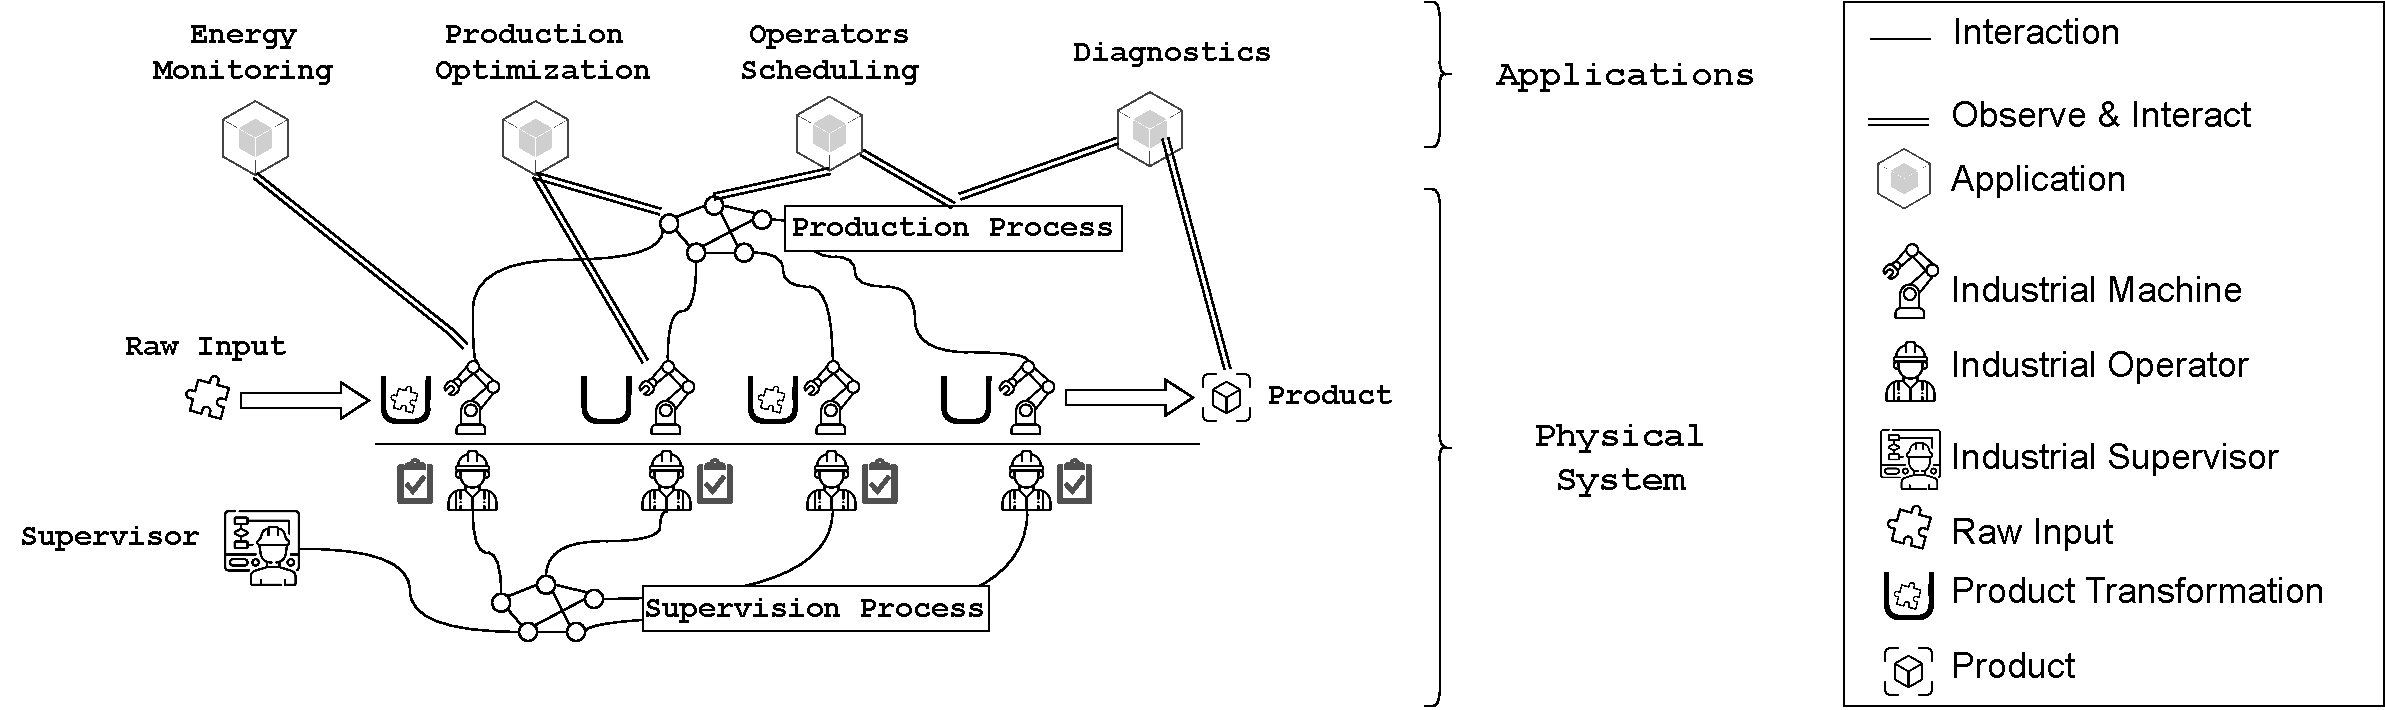
\includegraphics[width=\columnwidth]{figures/dt-mas/smart_manufacturing_scenario.pdf}
    \caption{A reference Smart Manufacturing scenario with multiple physical entities and a set of applications interested in implementing intelligent functionalities on top of the physical deployment.}
    \label{fig:smart_manufacturing_scenario}
\end{figure*}

%======================================================
\subsection{A Smart Manufacturing Energy Optimisation Scenario}
%======================================================

A typical production system distributes a diverse array of \textit{machinery}, \textit{operators}, and \textit{processes} throughout the shop-floor environment (as schematically represented in Figure \ref{fig:smart_manufacturing_scenario}). 
%These elements can be classified into various categories based on their nature and usage. For instance, there are feeding-material systems responsible for managing material input, transformation systems such as production machines or specialized equipment for processing, output material systems for managing material output, and various material handling equipment including robotic arms and industrial manipulators interacting with industrial operators during different phases.
%
These individual components are often organised into \textit{production nodes}, which serve as logical groupings of related machines.
Several nodes make up the overall production plant.

Industrial energy monitoring \cite{Ageed2021ASO, Cai2022ARO} and optimisation \cite{Hussain2021SmartAI} is a challenging task, especially in a distributed environment. 
There, such tasks might involve several processes, to selectively turn on different nodes when needed, depending on the external information about the energy cost, while keeping the production speed at an acceptable rate.
%
Given the hierarchical organization of the plant and the cyber-physical distribution of the system, this problem calls for a DI approach.

%We here sketch the main high-level requirements for a Smart Manufacturing scenario targeting energy optimization at the plant level.
As summarised in Figure \ref{fig:target_functions}, we decompose the main target of production optimisation into three objectives that could be strategic in the target scenario and that represent a useful reference to analyse and apply the design principles presented and proposed in this article.

We identify three main functionalities that concur to dynamically adjust production based on energy costs, to keep the overall consumption under a threshold. 
The IoT system must be able to collect information about the current energy consumption and needs of each production node through some form of \emph{energy monitoring}. Furthermore, to be able to dynamically adjust the loads in the production nodes, some form of \emph{intelligent coordination} is required to continuously optimise the utilisation of resources. Finally, the overall \emph{production optimisation} techniques are required to make high-level decisions that incorporate data from both individual production nodes and external sources.
These functionalities are an exemplification of decomposition that can be performed in the design process of an IoT system. In the following, we analyse each functionality in more detail and guide this analysis towards the definition of components that can implement the IoT system employing either DTs or AAs or a combination of the two.

\begin{figure*}
    \centering
    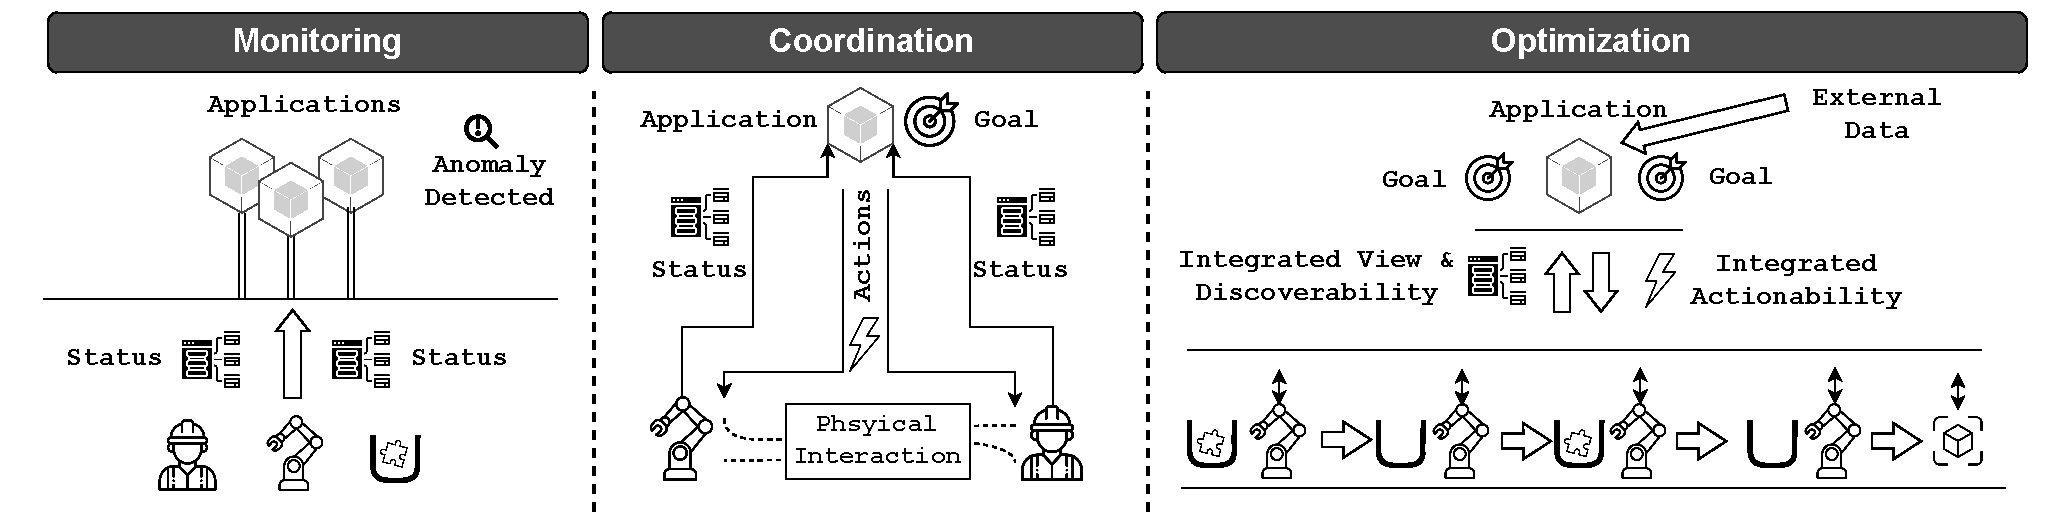
\includegraphics[width=\columnwidth]{figures/dt-mas/target_functions.pdf}
    \caption{Three main objectives that concur to the energy optimization of a Smart Manufacturing plant: Energy Monitoring at the machine level, Intelligent Coordination between robots and operators, and overall Production Optimization based on external factors (e.g. energy cost).}
    \label{fig:target_functions}
\end{figure*}

\paragraph{Energy Monitoring}
To make dynamic adjustments to the production process based on the energy consumption of the whole plant it is essential to be able to monitor it in real-time through smart metres embedded in the machines.
Furthermore, it is essential to collect data from each machine or production node to have fine-grained control on what parts of the plant are consuming the most energy.
%
Monitoring can also include some forms of inference to determine whether the observed consumption is considered regular or is an anomaly, and potentially take corrective actions in such cases to improve safety.
%
Finally, prediction or simulation can be used to forecast what the energy consumption is expected to be, given some production tasks, to improve decision-making.

\paragraph{Intelligent Coordination}
This objective involves the use of data collected from the IoT system to introduce coordination capabilities to improve both performance and safety at different levels of deployment (e.g., machine-to-machine or machine-to-operator interactions).
%
For example, machine learning models can be trained to detect patterns and, by continuously monitoring and analysing data streams from machines and operators, the system can automatically understand the context of the currently performed activities.
%
This is essential to understand the best planning policy to schedule the next tasks as soon as machines or operators are free to perform them.
%
%Furthermore, digital interfaces are required to interact with both robots and humans to assign tasks.
%
%For example, if an operator working is stressed or its fatigue level is anomaly increased, the coordination (intelligent) functionality can dynamically defer the assigned task or assign it to other operators.
%
For example, if a portion of the plant is to be shut down for energy saving, the tasks that were queued on those machines should be redistributed across the other active production nodes of the plant.

\paragraph{Production Optimisation}
Digital applications can combine real-time data from the physical world and external sources (e.g., market price and production demand) to dynamically optimise manufacturing processes together with all machines, operators, raw materials, and products.
%
This requires decision-making driven by inference of constraints, as well as means to monitor the current situation to adapt according to the real-time state of the system.
%
For this scenario, we assume that the market price of energy is provided by an external forecasting system. Based on that and according to target business rules, the digital layer can optimise production schedules, resource allocation, and task assignment to maximise efficiency and reduce costs.

\medskip
%The design and implementation of these outlined functionalities, along with other intelligent capabilities, must confront the reality of cyber-physical complexity. Bidirectional interaction with physical entities, their data, and actions poses a critical challenge for applications, necessitating delegation to an intermediate structured and interoperable digital level. This layer is tasked with decoupling these responsibilities from high-level applications.
In the subsequent section, we explore how AAs and DTs can be synergistically exploited to construct a cyber-physical intelligent abstraction layer following the design principles presented in Section \ref{ssec:principles}. %This layer aims to maximise interoperability, simplify interaction with physical entities, and facilitate the adoption of intelligent capabilities.

%======================================================
\subsection{System Design with AAs and DTs}
%======================================================
\label{ssec:system_design_aas_dts}

\note{TODO TABLE}
% \newcolumntype{P}[1]{>{\centering\arraybackslash}p{#1}}
% \newcolumntype{M}[1]{>{\centering\arraybackslash}m{#1}}
% \begin{table*}[!t]
%     \centering
%     \scriptsize
%     \begin{tabular}{ p{1.5cm} | p{2cm} p{1.5cm} P{1cm} P{1cm} P{1cm} P{1cm} P{1cm} }
%         \hline
%         \textbf{Overall Objective} & \textbf{Functionalities} & \textbf{Kind} & \textbf{Specif.} & \textbf{Scoping} & \textbf{Timing} & \textbf{Abst.} & \textbf{$\mu$-arch}\\
%         \hline
%         \multirow{3}{2cm}{Energy\\Monitoring} 
%         & Data collection & n.a. & General & Local & Explicit & DT & \multirow{3}*{E} \\ 
%         & \makecell[l]{Anomaly\\Detection} & \makecell[l]{Inference/\\Prediction} & General & Local & Explicit & DT & \\ 
%         & \makecell[l]{Corrective\\Reaction} & \makecell[l]{Inference/\\Planning} & Specific & Local & Implicit & Agent & \\
%         \hline
%         \multirow{3}{2cm}{Intelligent\\Coordination} 
%         & \makecell[l]{Activity\\Monitoring} & \makecell[l]{Inference/\\Prediction} & General & Local & Explicit & DT & \multirow{3}*{A}\\ 
%         & \makecell[l]{Dynamic\\Planning} & Planning & Specific & Global & Explicit & Agent &\\ 
%         & \makecell[l]{Task\\Delegation} & n.a. & General & Local & Implicit & DT &\\ 
%         \hline
%         \multirow{3}{2cm}{Production\\Optimization} 
%         & Decision-making & Inference & Specific & Global & Explicit & Agent & \multirow{3}*{A}\\ 
%         & \makecell[l]{Process\\Monitoring} & Inference & General & Global & Explicit & DT & \\ 
%         & \makecell[l]{Task\\Delegation} & n.a. & General & Local & Implicit & DT & \\ 
%         \hline
%     \end{tabular}
%     \caption{Mapping of design principles to the target use case and broad categories of intelligent functionalities (\rev{Specif.\ = Specificity, Abst.\ = Abstraction}, n.a.\ = not applicable, pure digitalization function).}
%     \label{tab:usecase_principles_mapping}
% \end{table*}


Table \ref{tab:usecase_principles_mapping} reports the mapping between the intelligence functionalities envisioned, the application of the design principles, and the associated micro-architectural design. % following the analysis with respect to the \textit{Specificity}, \textit{Scoping} and \textit{Timing} principles.
%
We decompose each overall objective into specific functionalities and associate them with the main \textit{ kinds} of intelligent functionalities identified in Section \ref{ssec:functions}.
%
The analysis leads to the adoption of an AA, a DT, or a combination thereof, for functionality, and a different $\mu$-arch for each objective (as shown in Figure \ref{fig:dt_agents_zoom}), choosing from those presented in Section \ref{ssec:multi-layer}.

In the following, we discuss the reasoning behind each choice, providing an illustrative interpretation of the principles for the different functionalities in the scenario presented above. 

\paragraph{Energy Monitoring}

For this objective, we identify the basic functionality of data collection about the energy consumption of a given machine. 
It has low specificity as the very same data required for the monitoring could easily and likely be used for other, future tasks (e.g., prediction of consumption). 
%
Of course, as the data belong (is both generated and consumed by) to a specific PA, the functionality is \textit{local} concerning the Scoping principle (actually, individual), 
%
and we consider an explicit time representation needed for this task to generate a time series. 

We also expect to have an anomaly detection functionality that can analyse time series data and detect unexpected patterns. 
The knowledge required for such a task is still local to the machine, and the results can be useful to general services as they could notify interested parties of a malfunction. 

Finally, we envision an on-the-fly corrective reaction mechanism that is introduced with the specific purpose of shutting down the machine if there is a problem. 
This is a specific behaviour introduced for our main monitoring application goal (hence, with application goal specificity), which still uses only the local data and can act on an event-driven trigger that does not necessarily need an explicit time representation. 

From this analysis, we can reliably identify the need for a machine DT, capable of collecting data and detecting anomalies, and of an AA implementing the emergency shutdown policy. 
This leads to $\mu$-arch \textbf{(E)} described in figure \ref{fig:architecture} as the possible reference implementation for this functionality. 

\begin{figure*}
    \centering
    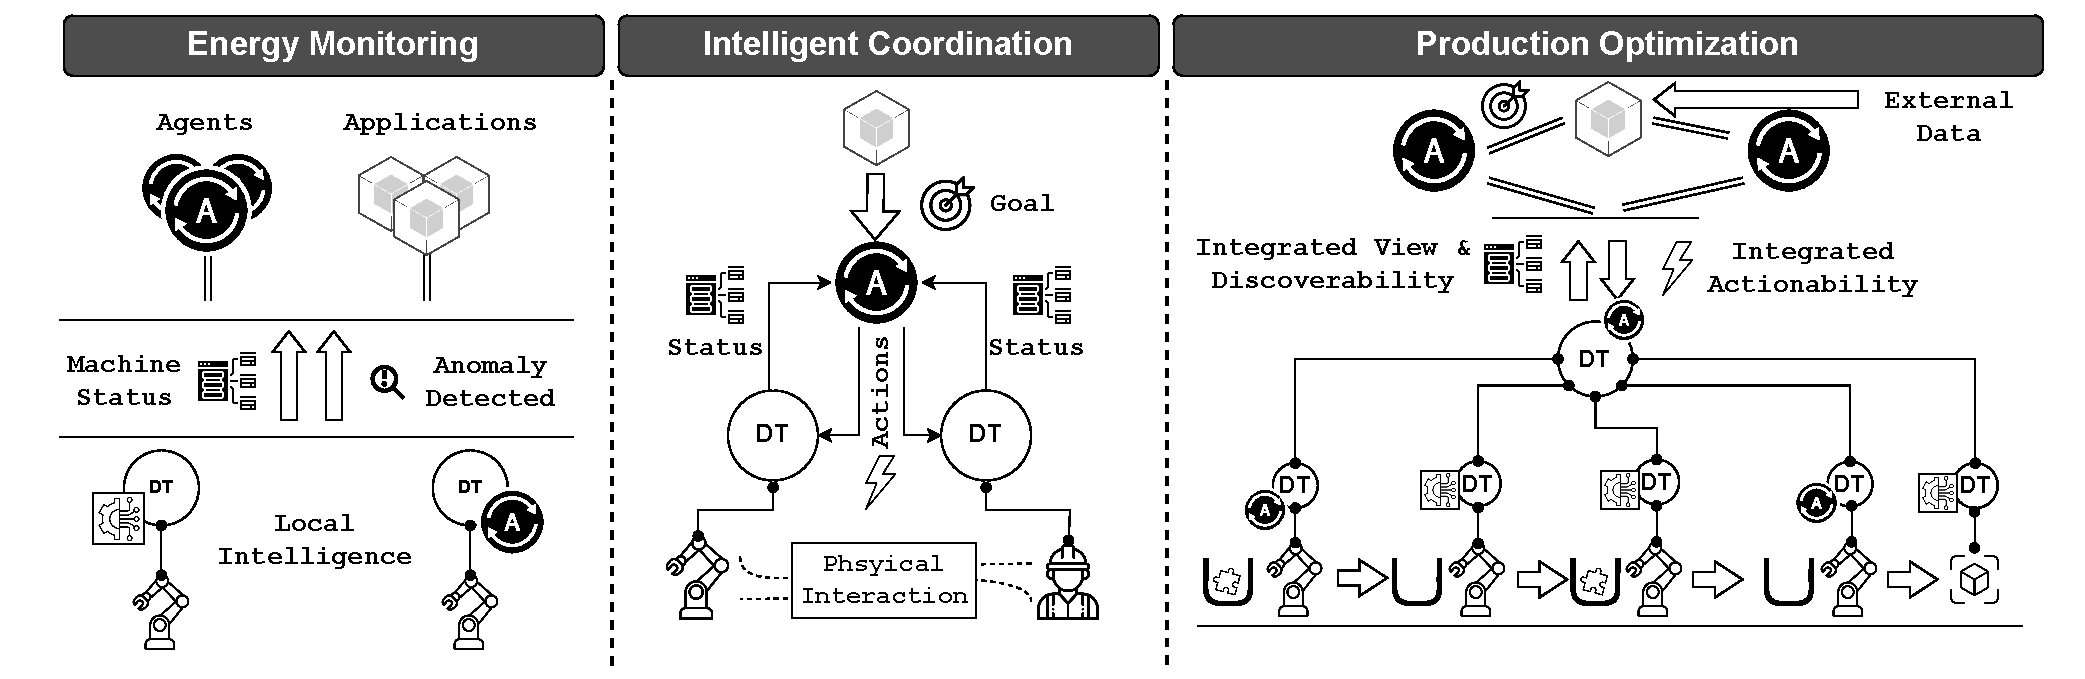
\includegraphics[width=\columnwidth]{figures/dt-mas/dt_agents_zoom.pdf}
    \caption{Three  illustrative instances showcasing the synergistic usage of AAs and DTs as guided by the principles and $\mu$-archs, within the Smart Manufacturing context.}
    \label{fig:dt_agents_zoom}
\end{figure*}

\paragraph{Intelligent Coordination}

The data necessary for this functionality comes from an activity monitoring task, which has \emph{local scope} on the PA being mirrored (e.g. an operator) to infer the activity currently executed and possibly predict the expected duration (thus, we an explicit representation of time needed, here). 
%
The function would be assigned from dynamic planning performed by another component of the system, after receiving the aggregated global knowledge (hence global scope) from each entity involved in the coordination scenario.

Accordingly, we may expect that each PA would have a DT that mirrors them and encapsulates the activity monitoring and task delegation functionalities, tailoring them to the mirrored entity. 
Planning, instead could be performed by an AA keeping track of the global context (e.g.\ of a whole production node) and applying a specific coordination policy to redirect tasks to different machines (hence, a functionality with goal specificity and global scope, justifying preference for an AA). 
This leads to the adoption of $\mu$-arch \textbf{(A)}, with a single agent using multiple DTs as its data sources and delegating tasks to each.

\paragraph{Production Optimisation}

Optimisation at the plant level will be guided by a decision-making functionality based on two sources of data: external data about the market price of electricity for a specific time and date
and data collected locally from the different production nodes. %that will need to feed into a global process monitoring functionality. 
%
Depending on the cost of electricity, for instance, the policy may decide to shut down the nodes that are not actively involved in the ongoing process, delegating tasks to different nodes.

Accordingly, $\mu$-arch \textbf{(A)} is the best suited in this scenario, involving a DT that mirrors the production process as the main data source, and an AA enacting the policy and acting on the production nodes.
%
It is worth noting that, having already introduced the DTs of the different production nodes, we can also consider linking the DT of the production process to the DTs of the nodes, in a composition pattern that would facilitate the modelling of the production process DT as represented in Figure \ref{fig:dt_agents_zoom}.

%======================================================
\subsection{Discussion of Resulting Architecture}
%======================================================

%In this section, we delve into the analysis of the integrated architecture and design choices concerning the use of DTs and Agents in the target manufacturing scenario, examining their respective advantages and disadvantages with respect also to the application of the envisioned design principles and the distribution of intelligent functionalities in the use case.

\begin{figure}[!b]
    \centering
    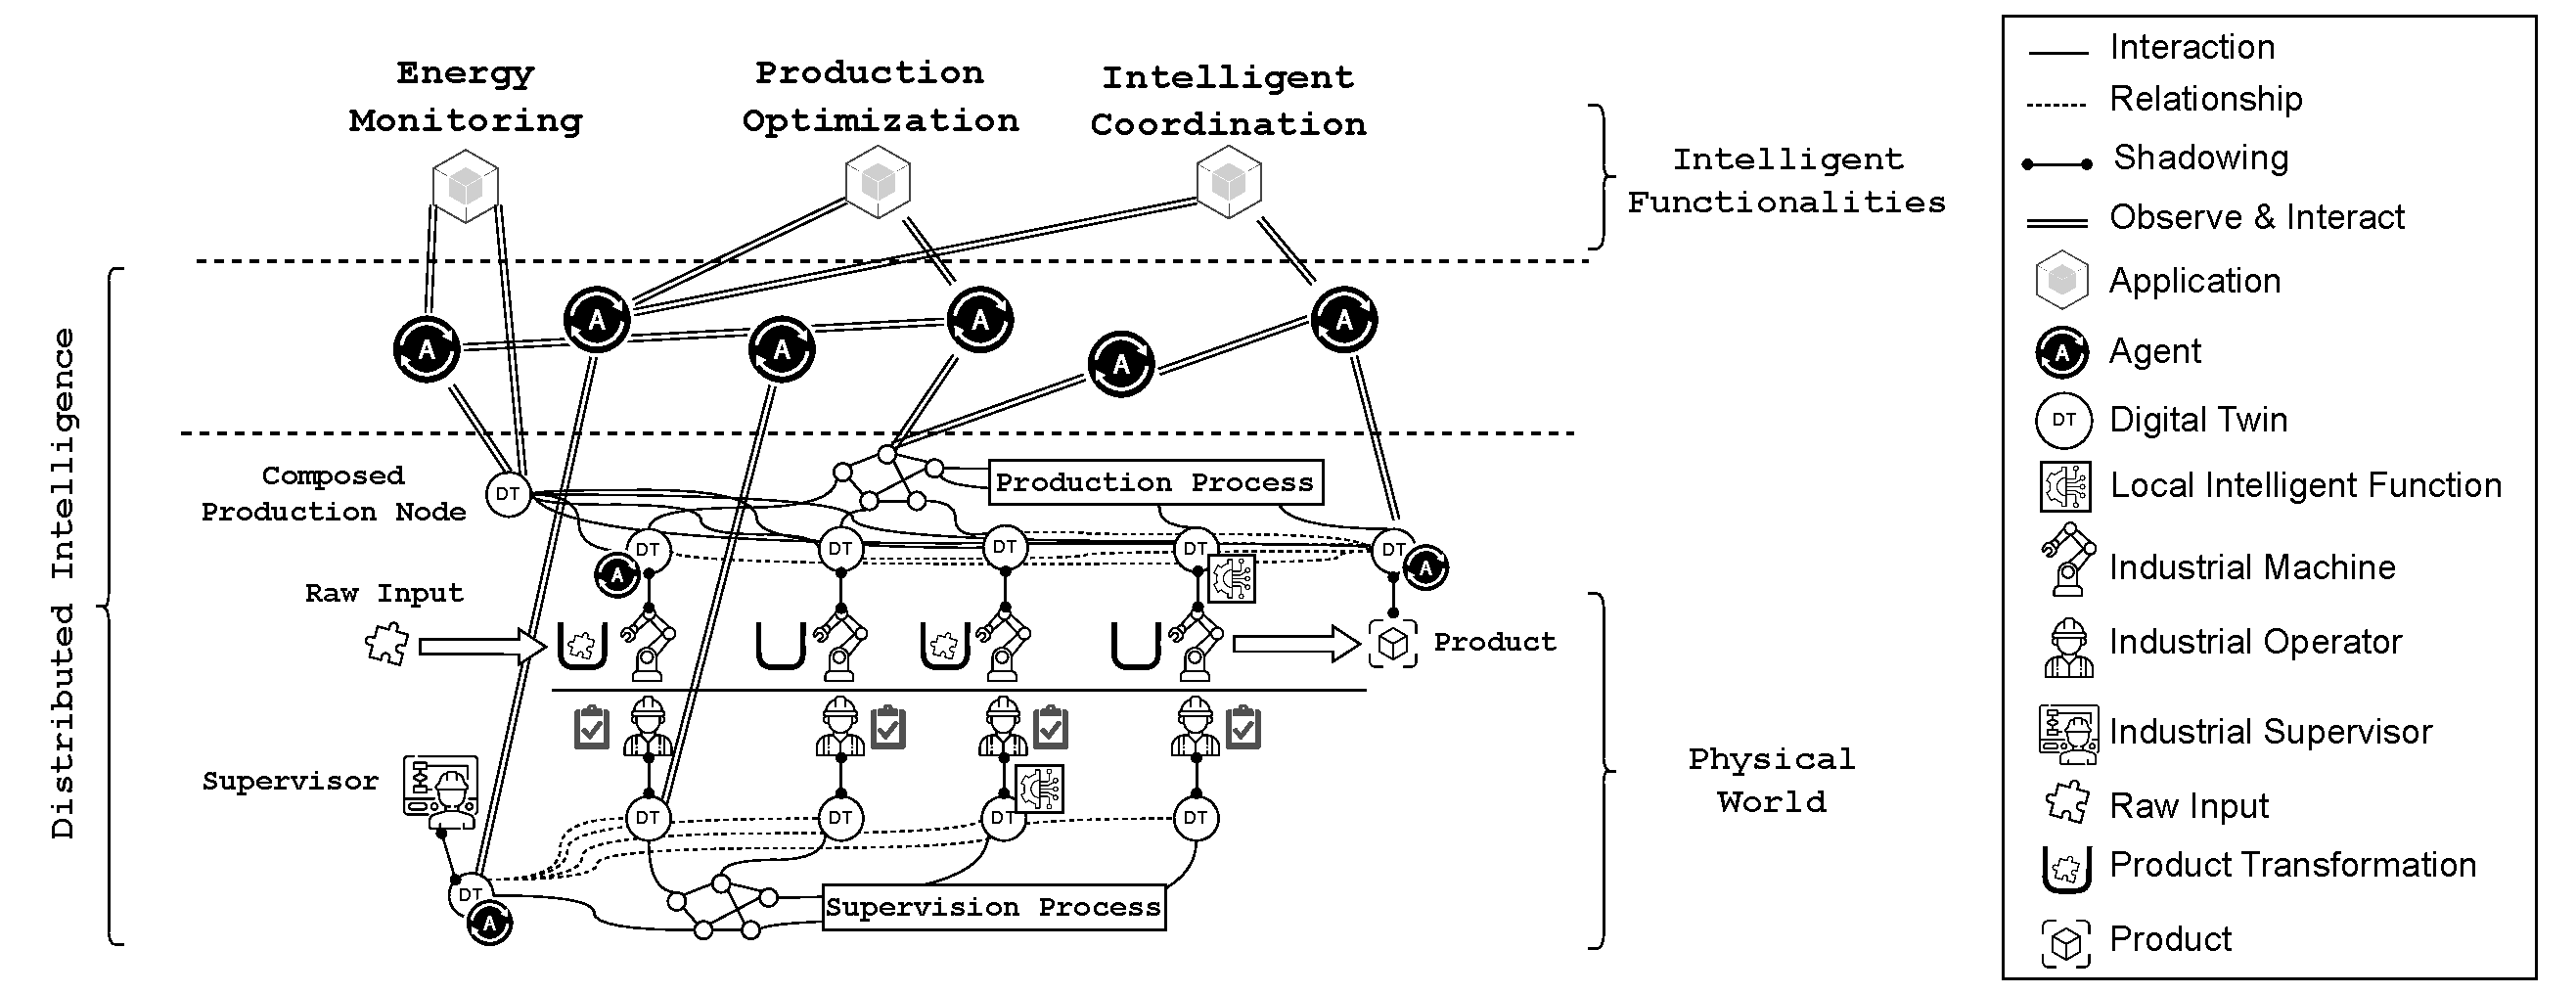
\includegraphics[width=\columnwidth]{figures/dt-mas/dt_agents_smart_manufacturing.pdf}
    \caption{A layered architecture with the combination of DTs and Agents for a Smart Manufacturing reference scenario.}
    \label{fig:dt_agents_smart_manufacturing}
\end{figure}

Figure \ref{fig:dt_agents_smart_manufacturing} schematically illustrates the integrated architecture, using both AAs and DTs, resulting from the application of our proposed design principles and the consequential composition of our $\mu$-archs. 
%The integrated architecture is emerging from the micro-patterns identified for each of the main objectives combined and as such leverages the strengths of both abstractions to create a robust, flexible, and intelligent manufacturing system where high-level intelligent functionalities are implemented using DTs and Agents according to their requirements and following principles and analysis presented in Section \ref{ssec:principles} and Section \ref{ssec:system_design_aas_dts}. 

The physical world, composed of multiple heterogeneous entities such as machines, operators, raw inputs, and products, can be effectively digitalised through the use of DTs.
These DTs are responsible for representing the associated PAs in cyberspace through interoperable and homogeneous digital replicas, operating locally to the devices and associated just to their context without the need for a global scope.
This approach can also be applied to industrial processes, such as product transformation from raw inputs to final products, the interaction and collaboration between machines and operators, etc.

DTs excel in abstracting and decoupling PAs and processes into modular digital representations, simplifying interaction and integration. They support standardized communication protocols, enhancing interoperability across various platforms and systems, that is critical for integrated manufacturing operations. DTs can be composed of higher-level aggregates, providing a holistic view of the system, which is crucial for understanding interdependencies and optimising system-wide processes.
%
Moreover, DTs can embed \emph{localized intelligence}, enabling real-time monitoring, anomaly detection, and predictive maintenance, while reducing latency and improving responsiveness.

On the other hand, AAs are designed to operate autonomously, making decisions based on predefined rules or learned behaviours, which allows them to adapt to changing conditions and respond effectively to real-time events. They excel in tasks requiring dynamic coordination and optimization, such as reallocating resources and adjusting schedules based on real-time data and system conditions. Additionally, AAs can be easily scaled and deployed across different parts of the manufacturing system, providing a flexible solution that can grow with the system's needs.
%
In the envisioned and reference smart manufacturing example, AAs can be distributed across the entire deployment spectrum. They support both local inference and decision-making within a DT, allowing it to achieve its internal target goals, and broader spectrum operations enabling dynamic coordination throughout the production line. This includes adapting planning and task allocation in response to variations in the production line context or external market demand. 
%In an intermediate approach, within a composed DT (e.g., operator supervisor), Agents enable the rebalancing of operator schedules and optimize the interaction among machines and operators.

AAs and DTs also benefit significantly from each other, in a perfect synergy. 
AAs benefit of DTs decoupling of complexity when interacting with the physical world and the exploitation of a uniform and interoperable digital representation of it. Conversely, AAs bring intelligence to the system, operating either internally as components of the DT's model (both for single and composed twins), or on a broader scope utilising the different DTs to collect information and act to improve overall performance and behaviour.
%
An additional benefit of such an integrated approach that combines both DTs and AAs is that the components can evolve separately.
%
Policies can change at the AA level (even online, via learning) without having to modify the DTs. 
Similarly, new and improved DT models could be produced as data is collected about the system, improving support given to the AA decision-making, without changing the AA at all. %but without requiring any kind of modification as the entities in the system are all loosely coupled. 

As a final remark, emphasising modularity, it is worth noting that in this example the decision-making is all performed by AAs. This means that in case of need (e.g.\ some critical failure or an expected contingency), to switch the system to a \textit{``manual mode''} it is sufficient to momentarily stop/disconnect the AAs. 
Then, they can be temporarily replaced by human operators to amend the system as needed, while still benefiting from the real-time data collected by DTs that can continue to operate. 

%Interaction mechanisms ensure bidirectional communication between DTs and Agents, enabling informed decision-making and action execution. The integration of DTs and Agents can significantly improve operational efficiency by enabling real-time monitoring, predictive maintenance, and dynamic optimization. Scalability is achieved through the proposed distributed architecture that allows for the addition of new DTs and Agents without disrupting existing operations. Flexibility ensures adaptability to changing conditions and requirements, maintaining resilience and responsiveness. 

All of these desirable non-functional properties do not come without costs: the next Section discuss the challenges that researchers and practitioners need to deal with to effectively adopt AAs and DTs according to our proposed principles and $\mu$-archs. %challenges include system integration, resource scaling, and initial deployment complexity, requiring careful planning and optimization strategies to overcome.
%The next Section discusses some of these.
%In conclusion, the combination of DTs and Agents in smart manufacturing provides a powerful framework for addressing the complexity and dynamic nature of modern production systems.
%Despite challenges, this integrated approach enhances operational efficiency, flexibility, and scalability, paving the way for future advancements in smart manufacturing.

%The integration of intelligent functionalities into smart manufacturing systems empowers organizations to achieve greater agility, responsiveness, and competitiveness in today's dynamic market landscape. These capabilities not only enhance operational efficiency and productivity but also elevate safety, quality, and sustainability throughout the entire manufacturing value chain. However, the design and implementation of these functionalities, along with other intelligent capabilities, must confront the reality of cyber-physical complexity. Bidirectional interaction with physical entities, their data, and actions poses a critical challenge for applications, necessitating delegation to an intermediate structured and interoperable digital level. This layer is tasked with decoupling these responsibilities from high-level applications. DTs and Agents can address these functionalities, constructing a new cyber-physical intelligent abstraction layer following the design principles presented in Section \ref{ssec:principles}. This layer aims to maximize interoperability, simplify interaction with physical entities, and facilitate the adoption of intelligent capabilities.

%In this context, interoperability is also another pivotal aspect of DT technology associated with the target operational scope of the physical asset, facilitating seamless communication and integration with various digital and physical protocols. This interoperability fosters collaboration and data exchange across different platforms, enhancing the efficiency and effectiveness of manufacturing processes. In terms of interaction with applications or services, DTs streamline communication through standardized protocols, enabling seamless integration with external systems. Applications and Agents can interact with DTs by requesting modifications to the state of affairs, pushing configurations and plans, and accessing information about physical assets and their capabilities through the DT structure. This capability results in strategy in combination with composition through all the greenified function categories since it enables a simplified and structured data collection from the DT and an effective actionability enabling agents to return to the physical world to change behaviours, coordinate and optimize processes.

%However, their integration with existing systems and protocols can be complex, requiring careful design and robust communication mechanisms to ensure seamless interaction with DTs and other system components.
%Autonomous agents can also be resource-intensive, particularly if they perform complex computations or require significant data exchange, potentially straining network and computational resources.

%The bottom layer consists of physical assets, while the middle layer is populated with DTs representing these assets, providing a digital abstraction that captures real-time data and historical performance. The top layer consists of Agents that utilize data from DTs to perform intelligent functions such as monitoring, coordination, and optimization.

